\documentclass{article}

\usepackage{blindtext}
\usepackage{multicol}
\usepackage{caption}
\usepackage{bm}
\usepackage{tikz}
\usepackage{pgfplots}
\usepackage{hyperref}
\hypersetup{
    colorlinks=true,
    linkcolor=blue,
    filecolor=magenta,      
    urlcolor=cyan,
}
\usepackage{geometry}
\geometry{
	a4paper,
	noheadfoot=true,
	left=1.0in,
	right=1.0in,
	top=1.0in,
	bottom=1.0in
}

% url package
\usepackage{hyperref}
\usepackage{subcaption}

% Titling and Author
\title{Latex Tikz Examples, Annotate on Graph}
\author{\href{https://fanwangecon.github.io/}{Fan Wang}\thanks{https://fanwangecon.github.io, repository: \href{https://fanwangecon.github.io/Tex4Econ/}{Tex4Econ}}}
\date{\today}

\begin{document}

\maketitle

\section{Annotate Text in Figure}

\subsection{Slope and Intercept Annotate}
 
Draw axis below, and a line, middle of page, and annotate the slope of the intercept with arrows. Annotate with box without color.

\begin{verbatim}
\begin{center}
\begin{tikzpicture}
\draw (0,2) -- (0.25*\textwidth,2);
\draw (0,1) -- (0.5*\textwidth,1);
\end{tikzpicture}
\end{center}
\end{verbatim}
\bigskip
\begin{center}
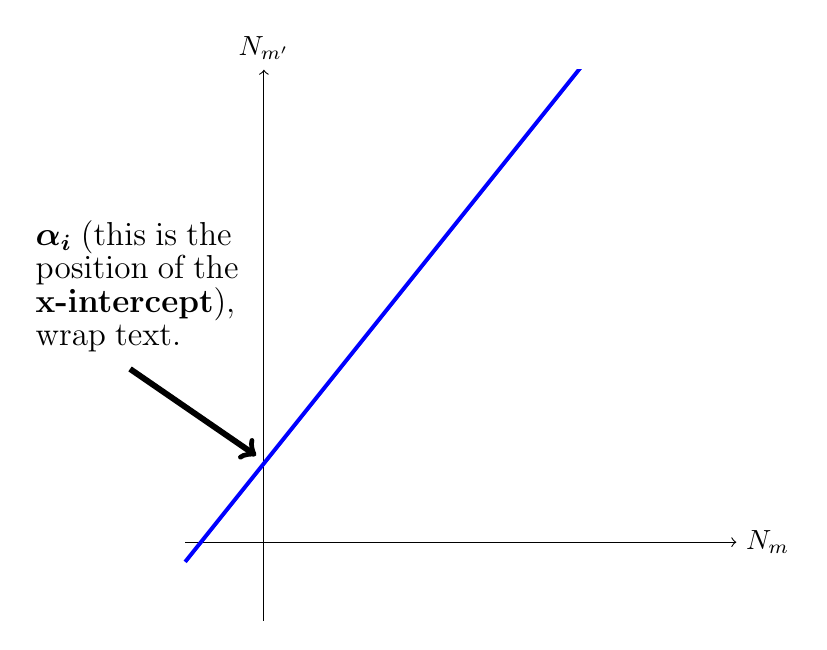
\begin{tikzpicture}
\draw[->] (-1,0) -- (6,0) node[right] {$N_m$};
\draw[->] (0,-1) -- (0,6) node[above] {$N_{m^{\prime}}$};

% A. Clip area so that line below is only drawn inside finite box
\clip (-3,-1) rectangle (6,6);

% B. Draw a line with intercept and slope
\draw[line width=0.50mm,domain=-1:6,smooth,variable=\x, blue] plot ({\x},{1+\x*1.25});

% C. Draw Line pointing to Intercept of line
\draw[->, line width=0.75mm] (-1.7,2.2) -- (-0.1,1.1);

% D. Draw a transparent text box that wraps text
\node[text width=3cm] at (-1.4,3.25) {\large{$\bm{\alpha_i}$ (this is the position of the \textbf{x-intercept}), wrap text.}};

\end{tikzpicture}
\end{center}




\end{document}